%==========================================================
% CHAPTER 2: Funkcijos išvestinė ir jos taikymas
%==========================================================
\chapter{Funkcijos išvestinė ir jos taikymas}

\section{Išvestinės apibrėžimas}

Diferencialinis skaičiavimas – viena iš pagrindinių matematinės analizės šakų, nagrinėjančių funkcijų kitimo greitį. Pagrindinis šios srities objektas yra \textbf{išvestinė} – skaičius, apibūdinantis, kaip greitai funkcijos reikšmė kinta ties konkrečiu argumentu.

\begin{definition}
Funkcijos $f$ \textbf{išvestine} taške $x_0$ vadinamas skaičius
\[
f'(x_0) = \lim_{\Delta x \to 0} \frac{f(x_0 + \Delta x) - f(x_0)}{\Delta x},
\]
jei ši riba egzistuoja ir yra baigtinė. Jei tokia riba egzistuoja, sakome, kad funkcija $f$ yra \textbf{diferencijuojama} taške $x_0$.
\end{definition}

Santykis $\dfrac{\Delta y}{\Delta x} = \dfrac{f(x_0+\Delta x)-f(x_0)}{\Delta x}$ vadinamas \textbf{diferencine išraiška} arba \textbf{sekantinės krypties koeficientu}. Kai $\Delta x \to 0$, sekantinė virsta liestine, o diferencinė išraiška artėja prie išvestinės reikšmės.

\medskip
Išvestinė žymima keliais būdais:
\[
f'(x_0), \quad y'(x_0), \quad \frac{dy}{dx}\bigg|_{x=x_0}, \quad \frac{df}{dx}\bigg|_{x=x_0}.
\]

\begin{remark}
Leibnico žymėjimas $\dfrac{dy}{dx}$ pabrėžia išvestinės kaip dviejų begalinai mažų dydžių $dy$ ir $dx$ santykio idėją – tai ypač naudinga diferencialų teorijoje.
\end{remark}

\subsection{Geometrinė prasmė}

Išvestinės geometrinė prasmė tiesiogiai susijusi su funkcijos grafiko \textbf{liestine}.

\begin{tcolorbox}[colback=blue!5!white, colframe=blue!60!black, title=Geometrinė išvestinės prasmė]
Jei funkcija $f(x)$ taške $x_0$ turi išvestinę, tai $f'(x_0)$ yra lygus kreivės $y = f(x)$ \textbf{liestinės krypties koeficientui} taške $M_0\bigl(x_0,\, f(x_0)\bigr)$:
\[
f'(x_0) = k = \tg\alpha,
\]
kur $\alpha$ – kampas tarp liestinės ir teigiamosios $Ox$ pusašės.
\end{tcolorbox}

\subsubsection*{Liestinės lygtis}

Žinant liestinės krypties koeficientą $k = f'(x_0)$ ir lietimosi tašką $M_0(x_0, f(x_0))$, liestinės lygtį užrašome naudodami tiesės lygtį per tašką su žinomu krypties koeficientu:

\[
\boxed{y - f(x_0) = f'(x_0)\cdot(x - x_0)}
\]

\begin{example}
Raskite funkcijos $f(x) = x^2$ grafiko liestinės lygtį taške $x_0 = 2$.

\textbf{Sprendimas.}
\begin{enumerate}
    \item Randame lietimosi taško koordinates: $f(2) = 4$, taigi $M_0(2;\,4)$.
    \item Randame išvestinę: $f'(x) = 2x$, vadinasi $f'(2) = 4$.
    \item Sudarome liestinės lygtį:
    \[
    y - 4 = 4(x - 2) \implies y = 4x - 4.
    \]
\end{enumerate}
\end{example}

\subsubsection*{Sekantinė ir liestinė}

Pažvelkime, kaip sekantinė virsta liestine. Paimkime du funkcijos grafiko taškus: $M_0(x_0, f(x_0))$ ir $M_1(x_0+\Delta x,\, f(x_0+\Delta x))$. Per juos einanti tiesė vadinama \textbf{sekantine}. Jos krypties koeficientas:

\[
k_{\text{sek}} = \frac{f(x_0 + \Delta x) - f(x_0)}{\Delta x} = \frac{\Delta y}{\Delta x}.
\]

Kai $\Delta x \to 0$, taškas $M_1$ artėja prie $M_0$, o sekantinė artėja prie \textbf{liestinės} kreivei taške $M_0$. Todėl:

\[
k_{\text{liest}} = \lim_{\Delta x \to 0} \frac{\Delta y}{\Delta x} = f'(x_0).
\]

\begin{center}
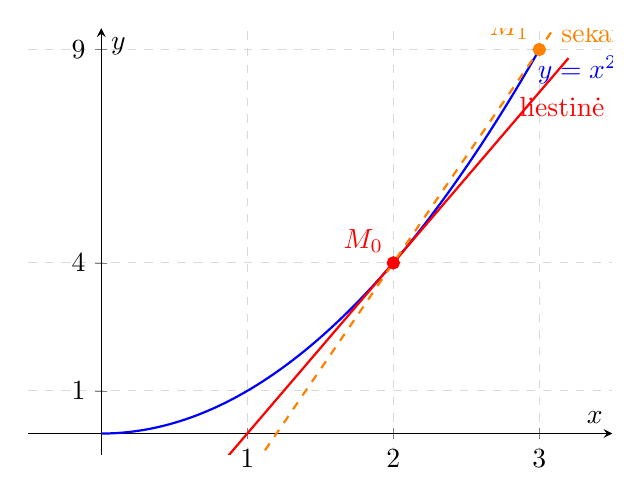
\begin{tikzpicture}
\begin{axis}[
    axis lines=middle,
    xlabel={$x$}, ylabel={$y$},
    xmin=-0.5, xmax=3.5,
    ymin=-0.5, ymax=9.5,
    xtick={1,2,3},
    ytick={1,4,9},
    width=9cm, height=7cm,
    grid=major,
    grid style={dashed, gray!30},
    every axis plot/.append style={thick}
]
% Parabola y = x^2
\addplot[blue, domain=0:3, samples=100] {x^2} node[right, pos=0.95] {$y=x^2$};

% Liestinė taške x0=2: y = 4x - 4
\addplot[red, domain=0.5:3.2] {4*x - 4} node[above right, pos=0.85] {liestinė};

% Sekantinė per (2,4) ir (3,9): šlaitumas = (9-4)/(3-2) = 5
\addplot[orange, dashed, domain=0.8:3.2] {5*x - 6} node[right, pos=0.95] {sekantinė};

% Taškai
\addplot[mark=*, mark size=2pt, red] coordinates {(2,4)} node[above left] {$M_0$};
\addplot[mark=*, mark size=2pt, orange] coordinates {(3,9)} node[above left] {$M_1$};

\end{axis}
\end{tikzpicture}
\end{center}

\subsubsection*{Ryšys tarp liestinės kampo ir išvestinės ženklo}

\begin{center}
\begin{tabular}{|c|c|c|}
\hline
\textbf{Sąlyga} & \textbf{Kampas} $\alpha$ & \textbf{Funkcijos elgsena} \\
\hline
$f'(x_0) > 0$ & $\alpha \in \left(0°;\,90°\right)$ & Funkcija didėja taške $x_0$ \\
$f'(x_0) < 0$ & $\alpha \in \left(90°;\,180°\right)$ & Funkcija mažėja taške $x_0$ \\
$f'(x_0) = 0$ & $\alpha = 0°$ & Liestinė lygiagreti $Ox$ ašiai \\
$f'(x_0)$ neegzistuoja & – & Funkcija nediferencijuojama taške $x_0$ \\
\hline
\end{tabular}
\end{center}

\begin{exercise}
Kreivės $y = x^3 - 3x + 1$ grafike raskite taškus, kuriuose liestinė yra lygiagreti $Ox$ ašiai.

\textbf{Sprendimas.} Liestinė lygiagreti $Ox$ ašiai, kai $y' = 0$.
\[
y' = 3x^2 - 3 = 0 \implies x^2 = 1 \implies x = \pm 1.
\]
Taškuose $x = 1$: $y(1) = 1 - 3 + 1 = -1$, ir $x = -1$: $y(-1) = -1 + 3 + 1 = 3$.

Atsakymas: taškai $(1;\,-1)$ ir $(-1;\,3)$.
\end{exercise}

\subsection{Fizinė prasmė}

Išvestinė fizikoje interpretuojama kaip \textbf{momentinis greitis} – dydis, apibūdinantis, kaip greitai kinta vienas fizikinis dydis, kintant kitam.

\begin{tcolorbox}[colback=green!5!white, colframe=green!60!black, title=Fizinė išvestinės prasmė]
Jei $S(t)$ – kūno nueitas kelias per laiką $t$, tai kūno \textbf{momentinis greitis} laiko momentu $t_0$ yra:
\[
v(t_0) = S'(t_0) = \lim_{\Delta t \to 0} \frac{S(t_0 + \Delta t) - S(t_0)}{\Delta t} = \lim_{\Delta t \to 0}\frac{\Delta S}{\Delta t}.
\]
\end{tcolorbox}

\subsubsection*{Vidutinis ir momentinis greitis}

Santykis $\bar{v} = \dfrac{\Delta S}{\Delta t}$ vadinamas \textbf{vidutiniu greičiu} laiko intervale $[t_0,\, t_0 + \Delta t]$. Jis apibūdina bendrą judėjimo intensyvumą, tačiau neatskleidžia greičio pokyčių konkrečiu momentu. Kai laiko intervalas traukiamas į nulį:
\[
v(t_0) = \lim_{\Delta t \to 0} \bar{v} = S'(t_0),
\]
gauname \textbf{momentinį greitį} – tikslų greičio įvertį laiko momentu $t_0$.

\subsubsection*{Pagreitis}

Analogiškai, jei $v(t)$ – kūno greitis laiku $t$, tai \textbf{momentinis pagreitis} apibrėžiamas kaip greičio išvestinė laiko atžvilgiu:
\[
a(t_0) = v'(t_0) = S''(t_0).
\]
Taigi pagreitis yra antroji kelio funkcijos išvestinė laiko atžvilgiu.

\subsubsection*{Kiti fiziniai taikymai}

Išvestinės sąvoka naudojama daugelyje fizikos sričių:

\begin{itemize}
    \item \textbf{Elektra:} Srovės stiprumas $I(t) = Q'(t)$, kur $Q(t)$ – per laidininką pratekėjęs krūvis.
    \item \textbf{Šiluma:} Šiluminės galios pokyčio greitis: $P = W'(t)$, kur $W(t)$ – energija.
    \item \textbf{Chemija:} Reakcijos greitis: $w = \dfrac{d[\text{C}]}{dt}$, kur $[\text{C}]$ – medžiagos koncentracija.
    \item \textbf{Biologija:} Populiacijos augimo greitis: $r = N'(t)$, kur $N(t)$ – individų skaičius.
\end{itemize}

\begin{example}
Automobilis juda pagal dėsnį $S(t) = 5t^2 + 3t$ (metrais, sekundėmis). Raskite:
\begin{enumerate}[label=\alph*)]
    \item Momentinį greitį laiko momentu $t_0 = 4\,\text{s}$.
    \item Pagreitį.
\end{enumerate}

\textbf{Sprendimas.}
\begin{enumerate}[label=\alph*)]
    \item $v(t) = S'(t) = 10t + 3$, todėl $v(4) = 10 \cdot 4 + 3 = 43\,\text{m/s}$.
    \item $a(t) = v'(t) = S''(t) = 10\,\text{m/s}^2$ (pastovus pagreitis).
\end{enumerate}
\end{example}

\begin{exercise}
Kūno judėjimo lygtis $S(t) = t^3 - 6t^2 + 9t$ (SI vienetai).
\begin{enumerate}[label=\alph*)]
    \item Raskite kūno greitį laiko momentais $t = 1$ ir $t = 3$.
    \item Kuriais laiko momentais kūnas sustoja (greitis lygus nuliui)?
    \item Raskite pagreitį, kai $t = 2$.
\end{enumerate}

\textbf{Sprendimas.}
\begin{enumerate}[label=\alph*)]
    \item $v(t) = S'(t) = 3t^2 - 12t + 9$.\\
          $v(1) = 3 - 12 + 9 = 0\,\text{m/s}$; \quad $v(3) = 27 - 36 + 9 = 0\,\text{m/s}$.
    \item $3t^2 - 12t + 9 = 0 \implies t^2 - 4t + 3 = 0 \implies (t-1)(t-3) = 0$.\\
          Kūnas sustoja momentais $t = 1\,\text{s}$ ir $t = 3\,\text{s}$.
    \item $a(t) = v'(t) = 6t - 12$; \quad $a(2) = 12 - 12 = 0\,\text{m/s}^2$.
\end{enumerate}
\end{exercise}


\section{Išvestinių skaičiavimo taisyklės}

% =========================================================
\subsection{Pagrindinės funkcijų išvestinės}
% =========================================================

Žemiau pateikiamos pagrindinių elementariųjų funkcijų išvestinės, kurias būtina
žinoti rengiantis VBE. Jos yra išvedamos tiesiogiai iš išvestinės apibrėžimo ir
sudaro visų sudėtingesnių skaičiavimų pagrindą.

\begin{tcolorbox}[title={Pagrindinių funkcijų išvestinių lentelė}, colback=blue!5, colframe=blue!40!black]
\begin{center}
\renewcommand{\arraystretch}{1.8}
\begin{tabular}{|c|c||c|c|}
\hline
\textbf{Funkcija} $f(x)$ & \textbf{Išvestinė} $f'(x)$ & \textbf{Funkcija} $f(x)$ & \textbf{Išvestinė} $f'(x)$ \\
\hline
$C$ (konstanta) & $0$ & $\sin x$ & $\cos x$ \\
\hline
$x$ & $1$ & $\cos x$ & $-\sin x$ \\
\hline
$x^n$ & $n x^{n-1}$ & $\tg\, x$ & $\dfrac{1}{\cos^2 x}$ \\
\hline
$\sqrt{x}$ & $\dfrac{1}{2\sqrt{x}}$ & $e^x$ & $e^x$ \\
\hline
$\dfrac{1}{x}$ & $-\dfrac{1}{x^2}$ & $a^x$ & $a^x \ln a$ \\
\hline
$\ln x$ & $\dfrac{1}{x}$ & $\log_a x$ & $\dfrac{1}{x \ln a}$ \\
\hline
\end{tabular}
\end{center}
\end{tcolorbox}

\begin{remark}
Laipsnio taisyklė $(x^n)' = nx^{n-1}$ galioja visiems realiesiems $n$, taip pat ir
trupmeniniams bei neigiamams laipsniams:
\[
\left(\sqrt{x}\right)' = \left(x^{1/2}\right)' = \frac{1}{2}\,x^{-1/2} = \frac{1}{2\sqrt{x}}, \qquad
\left(\frac{1}{x}\right)' = \left(x^{-1}\right)' = -x^{-2} = -\frac{1}{x^2}.
\]
\end{remark}

\begin{example}
Suraskite funkcijų išvestines:
\begin{enumerate}[label=\alph*)]
    \item $f(x) = x^5$
    \item $f(x) = \sqrt[3]{x^2}$
    \item $f(x) = 3^x$
    \item $f(x) = \log_2 x$
\end{enumerate}

\textbf{Sprendimai:}
\begin{enumerate}[label=\alph*)]
    \item Taikome laipsnio taisyklę:
    \[
        f'(x) = 5x^{5-1} = 5x^4.
    \]
    \item Perrašome kaip laipsnį: $f(x) = x^{2/3}$, tada
    \[
        f'(x) = \frac{2}{3}\,x^{2/3\,-1} = \frac{2}{3}\,x^{-1/3} = \frac{2}{3\sqrt[3]{x}}.
    \]
    \item Taikome rodiklinės funkcijos formulę:
    \[
        f'(x) = 3^x \ln 3.
    \]
    \item Taikome logaritminės funkcijos formulę:
    \[
        f'(x) = \frac{1}{x \ln 2}.
    \]
\end{enumerate}
\end{example}

% =========================================================
\subsection{Sudėties, sandaugos ir dalinimo taisyklės}
% =========================================================

Kai funkcija yra sudaryta iš kelių paprastesnių funkcijų algebrinių veiksmų,
naudojamos šios trys taisyklės.

\begin{tcolorbox}[title={Skaičiavimo taisyklės}, colback=green!5, colframe=green!40!black]
Tegu $f(x)$ ir $g(x)$ yra diferencijuojamos funkcijos, o $C$ --- konstanta. Tada:

\medskip
\textbf{1. Sumos (skirtumo) taisyklė:}
\[
    \bigl(f(x) \pm g(x)\bigr)' = f'(x) \pm g'(x).
\]

\textbf{2. Konstantos ir funkcijos sandaugos taisyklė:}
\[
    \bigl(C \cdot f(x)\bigr)' = C \cdot f'(x).
\]

\textbf{3. Sandaugos taisyklė:}
\[
    \bigl(f(x) \cdot g(x)\bigr)' = f'(x)\cdot g(x) + f(x)\cdot g'(x).
\]

\textbf{4. Dalinimo taisyklė} (kai $g(x)\neq 0$):
\[
    \left(\frac{f(x)}{g(x)}\right)' = \frac{f'(x)\cdot g(x) - f(x)\cdot g'(x)}{\bigl[g(x)\bigr]^2}.
\]
\end{tcolorbox}

\begin{remark}
Dalinimo taisyklėje \textbf{tvarka skaitiklyje yra svarbi}: pirmiausia rašomas
pirmosios funkcijos išvestinė, padauginta iš antrosios, \textit{minus} pirmoji funkcija,
padauginta iš antrosios išvestinės.
\end{remark}

\begin{example}
Apskaičiuokite funkcijos $f(x) = 3x^4 - 5x^2 + 7x - 2$ išvestinę.

\textbf{Sprendimas.} Taikome sumos ir konstantos taisykles kiekvienam dėmeniui atskirai:
\[
    f'(x) = 3\cdot 4x^3 - 5\cdot 2x + 7\cdot 1 - 0 = 12x^3 - 10x + 7.
\]
\end{example}

\begin{example}
Suraskite funkcijos $f(x) = x^3 \cdot \sin x$ išvestinę.

\textbf{Sprendimas.} Taikome sandaugos taisyklę, kur $u = x^3$, $v = \sin x$:
\[
    f'(x) = (x^3)' \cdot \sin x + x^3 \cdot (\sin x)' = 3x^2 \sin x + x^3 \cos x.
\]
\end{example}

\begin{example}
Suraskite funkcijos
\[
    f(x) = \frac{x^2 + 1}{x - 3}
\]
išvestinę.

\textbf{Sprendimas.} Pažymime $u = x^2+1$, $v = x-3$. Tada $u' = 2x$, $v' = 1$.
Taikome dalinimo taisyklę:
\[
    f'(x) = \frac{2x(x-3) - (x^2+1)\cdot 1}{(x-3)^2}
           = \frac{2x^2 - 6x - x^2 - 1}{(x-3)^2}
           = \frac{x^2 - 6x - 1}{(x-3)^2}.
\]
\end{example}

\begin{example}
Suraskite funkcijos $f(x) = e^x \cos x$ išvestinę ir apskaičiuokite $f'(0)$.

\textbf{Sprendimas.} Sandaugos taisyklė duoda:
\[
    f'(x) = (e^x)' \cos x + e^x (\cos x)' = e^x \cos x - e^x \sin x = e^x(\cos x - \sin x).
\]
Tada:
\[
    f'(0) = e^0(\cos 0 - \sin 0) = 1\cdot(1 - 0) = 1.
\]
\end{example}

\begin{exercise}
Apskaičiuokite šių funkcijų išvestines:
\begin{enumerate}[label=\arabic*.]
    \item $f(x) = 5x^3 - \dfrac{2}{x} + \sqrt{x}$
    \item $f(x) = (x^2 - 3)(2x + 1)$
    \item $f(x) = \dfrac{\sin x}{x}$
    \item $f(x) = x^2 \ln x$
    \item $f(x) = \dfrac{2x - 1}{x^2 + 4}$
\end{enumerate}
\end{exercise}

% =========================================================
\subsection{Sudėtinės funkcijos išvestinė (A kursas)}
% =========================================================

Dažnai funkcija yra sudaryta taip, kad vienos funkcijos argumentas yra kita
funkcija. Tokią funkciją vadiname \textbf{sudėtine funkcija} (angl.\ \textit{composite function}).

\begin{definition}
Jeigu $y = f(u)$ ir $u = g(x)$, tai funkcija
\[
    y = f\bigl(g(x)\bigr)
\]
vadinama \textbf{sudėtine funkcija}, kurioje $g(x)$ --- \textit{vidinė funkcija},
o $f$ --- \textit{išorinė funkcija}.
\end{definition}

\begin{tcolorbox}[title={Sudėtinės funkcijos išvestinė (grandinės taisyklė)},
                  colback=orange!5, colframe=orange!60!black]
Jeigu $u = g(x)$ yra diferencijuojama funkcija taške $x$, o $f$ yra diferencijuojama
taške $u = g(x)$, tai sudėtinės funkcijos $y = f(g(x))$ išvestinė:
\[
    \bigl[f\bigl(g(x)\bigr)\bigr]' = f'\bigl(g(x)\bigr)\cdot g'(x).
\]
Žodžiais: \textit{išorinės funkcijos išvestinė (su vidine funkcija viduje), padauginta
iš vidinės funkcijos išvestinės.}
\end{tcolorbox}

Praktinė schema: $\bigl(\text{išorinė}(\text{vidinė})\bigr)' = \text{išorinės iš.}(\text{vidinė}) \cdot \text{vidinės iš.}$

\medskip
Dažniausiai VBE pasitaikančios sudėtinių funkcijų formulės:

\begin{tcolorbox}[colback=yellow!5, colframe=yellow!60!black]
\[
    (u^n)' = n\,u^{n-1}\cdot u', \qquad
    (\sqrt{u})' = \frac{u'}{2\sqrt{u}},
\]
\[
    (e^u)' = e^u \cdot u', \qquad
    (a^u)' = a^u \ln a \cdot u',
\]
\[
    (\ln u)' = \frac{u'}{u}, \qquad
    (\log_a u)' = \frac{u'}{u \ln a},
\]
\[
    (\sin u)' = \cos u \cdot u', \qquad
    (\cos u)' = -\sin u \cdot u', \qquad
    (\tg\,u)' = \frac{u'}{\cos^2 u}.
\]
\end{tcolorbox}

\begin{example}
Suraskite funkcijos $f(x) = \sin(3x^2 - 1)$ išvestinę.

\textbf{Sprendimas.}
\begin{itemize}
    \item Išorinė funkcija: $\sin(\,\cdot\,)$, jos išvestinė: $\cos(\,\cdot\,)$.
    \item Vidinė funkcija: $u = 3x^2 - 1$, jos išvestinė: $u' = 6x$.
\end{itemize}
Taikome grandinės taisyklę:
\[
    f'(x) = \cos(3x^2-1) \cdot 6x = 6x\cos(3x^2-1).
\]
\end{example}

\begin{example}
Suraskite funkcijos $f(x) = e^{2x+5}$ išvestinę.

\textbf{Sprendimas.} Vidinė funkcija $u = 2x+5$, $u' = 2$. Todėl:
\[
    f'(x) = e^{2x+5}\cdot 2 = 2e^{2x+5}.
\]
\end{example}

\begin{example}
Raskite funkcijos $f(x) = \sqrt{x^2 + 4x - 1}$ išvestinę.

\textbf{Sprendimas.} Vidinė funkcija $u = x^2+4x-1$, $u' = 2x+4$. Todėl:
\[
    f'(x) = \frac{(2x+4)}{2\sqrt{x^2+4x-1}} = \frac{x+2}{\sqrt{x^2+4x-1}}.
\]
\end{example}

\begin{example}
Suraskite funkcijos $f(x) = \ln(\sin x)$ išvestinę.

\textbf{Sprendimas.} Vidinė funkcija $u = \sin x$, $u' = \cos x$. Todėl:
\[
    f'(x) = \frac{\cos x}{\sin x} = \ctg\, x.
\]
\end{example}

\begin{example}[Sudėtinė ir sandaugos taisyklė kartu]
Suraskite funkcijos $f(x) = x^2 \cdot e^{3x}$ išvestinę.

\textbf{Sprendimas.} Reikia taikyti ir sandaugos, ir grandinės taisykles.
Pažymime $u = x^2$, $v = e^{3x}$. Tada $u' = 2x$, o $v' = e^{3x}\cdot 3 = 3e^{3x}$.
Sandaugos taisyklė:
\[
    f'(x) = 2x \cdot e^{3x} + x^2 \cdot 3e^{3x} = e^{3x}(2x + 3x^2) = xe^{3x}(2 + 3x).
\]
\end{example}

\begin{exercise}
Apskaičiuokite šių sudėtinių funkcijų išvestines:
\begin{enumerate}[label=\arabic*.]
    \item $f(x) = (3x - 2)^5$
    \item $f(x) = \cos(x^3 + 1)$
    \item $f(x) = e^{-x^2}$
    \item $f(x) = \ln(x^2 + 1)$
    \item $f(x) = \sqrt[3]{2x^2 - 5}$
    \item $f(x) = \tg(5x)$
    \item $f(x) = 2^{\sin x}$
    \item $f(x) = \sin^3 x$ \quad \textit{(užuomina: perrašykite kaip $(\sin x)^3$)}
\end{enumerate}
\end{exercise}

\begin{tcolorbox}[title={Svarbi pastaba VBE}, colback=red!5, colframe=red!60!black]
Egzamine dažnai reikia \textbf{atpažinti sudėtinę funkciją} ir teisingai nustatyti
vidinę bei išorinę dalis. Tipinė klaida --- pamiršti padauginti iš vidinės funkcijos
išvestinės $u'$. Pavyzdžiui:
\[
    (\sin(2x))' = \cos(2x)\cdot\underbrace{2}_{\text{vidinės iš.}} = 2\cos(2x),
    \quad \text{o \textbf{ne} } \cos(2x).
\]
\end{tcolorbox}

\section{Funkcijos tyrimas naudojant išvestinę}

Išvestinė yra viena iš galingiausių analizės priemonių, leidžiančių nustatyti
funkcijos elgseną: kur ji didėja ar mažėja, kur pasiekia ekstremumus ir kaip
atrodo jos grafiko liestinė konkrečiame taške.

% ----------------------------------------------------------------
\subsection{Funkcijos monotoniškumas}
% ----------------------------------------------------------------

\begin{definition}
Funkcija $f$ vadinama \textbf{didėjančia} intervale $(a,b)$, jei kiekvienai
porai $x_1, x_2 \in (a,b)$, kuriai $x_1 < x_2$, galioja $f(x_1) < f(x_2)$.
Funkcija vadinama \textbf{mažėjančia} intervale $(a,b)$, jei iš $x_1 < x_2$
seka $f(x_1) > f(x_2)$.
\end{definition}

\begin{theorem}[Monotoniškumo kriterijus]
Tarkime, funkcija $f$ yra diferencijuojama intervale $(a,b)$.
\begin{enumerate}
  \item Jei $f'(x) > 0$ visiems $x \in (a,b)$, tai $f$ \textbf{didėja}
        intervale $(a,b)$.
  \item Jei $f'(x) < 0$ visiems $x \in (a,b)$, tai $f$ \textbf{mažėja}
        intervale $(a,b)$.
  \item Jei $f'(x) = 0$ visiems $x \in (a,b)$, tai $f$ yra \textbf{pastovi}
        (konstanta) intervale $(a,b)$.
\end{enumerate}
\end{theorem}

\begin{remark}
Atskiri taškai, kuriuose $f'(x) = 0$, nenutraukia funkcijos monotoniškumo
intervalo. Pavyzdžiui, $f(x) = x^3$ yra didėjanti visoje $\mathbb{R}$,
nors $f'(0) = 0$.
\end{remark}

\subsubsection*{Didėjimo ir mažėjimo intervalų radimo algoritmas}

\begin{enumerate}
  \item Apskaičiuokite $f'(x)$.
  \item Išspręskite lygtį $f'(x) = 0$ ir raskite taškus, kuriuose $f'(x)$
        neegzistuoja.
  \item Gautus taškus (kritinius taškus) sužymėkite ant skaičių ašies --
        jie suskaido apibrėžimo sritį į intervalus.
  \item Kiekviename intervale patikrinkite $f'(x)$ ženklą (pakanka paimti
        vieną bandomąją reikšmę).
  \item Užrašykite didėjimo ($f'>0$) ir mažėjimo ($f'<0$) intervalus.
\end{enumerate}

\begin{example}
Raskite funkcijos $f(x) = x^3 - 3x^2 - 9x + 5$ didėjimo ir mažėjimo
intervalus.

\textbf{Sprendimas.}
\[
  f'(x) = 3x^2 - 6x - 9 = 3(x^2 - 2x - 3) = 3(x-3)(x+1).
\]
Kritiniai taškai: $x_1 = -1$, $x_2 = 3$.

\medskip
\begin{center}
\begin{tabular}{c|ccccc}
  $x$     & $(-\infty;{-1})$ & $-1$ & $(-1;3)$ & $3$ & $(3;{+\infty})$ \\
  \hline
  $f'(x)$ & $+$              & $0$  & $-$      & $0$ & $+$             \\
  $f(x)$  & $\nearrow$       &      & $\searrow$&    & $\nearrow$      \\
\end{tabular}
\end{center}
\medskip

Funkcija \textbf{didėja}: $(-\infty;\,-1)$ ir $(3;\,+\infty)$.\\
Funkcija \textbf{mažėja}: $(-1;\,3)$.
\end{example}

% ----------------------------------------------------------------
\subsection{Funkcijos ekstremumai}
% ----------------------------------------------------------------

\begin{definition}
Taškas $x_0$ vadinamas funkcijos $f$ \textbf{kritiniu tašku}, jei
$f'(x_0) = 0$ arba $f'(x_0)$ neegzistuoja.
\end{definition}

\begin{definition}
Sakome, kad funkcija $f$ turi \textbf{lokalųjį maksimumą} taške $x_0$,
jei egzistuoja tokia aplinka $(x_0-\delta,\, x_0+\delta)$, kad
$f(x) \leq f(x_0)$ visiems $x$ toje aplinkoje.
Analogiškai apibrėžiamas \textbf{lokalusis minimumas}: $f(x) \geq f(x_0)$.
Bendras terminas -- \textbf{lokalusis ekstremumo taškas} (arba tiesiog
\emph{ekstremumo taškas}).
\end{definition}

\begin{theorem}[Būtina ekstremumo sąlyga]
Jei diferencijuojama funkcija $f$ turi lokaliąjį ekstremumą taške $x_0$,
tai $f'(x_0) = 0$.
\end{theorem}

\begin{remark}
Atvirkštinis teiginys nebūtinai teisingas: $f'(x_0)=0$ negarantuoja
ekstremumo. Pavyzdžiui, $f(x)=x^3$ -- $f'(0)=0$, tačiau taške $x=0$
ekstremumo nėra.
\end{remark}

\begin{theorem}[Pakankama ekstremumo sąlyga -- pirmoji išvestinė]
Tarkime, $x_0$ yra funkcijos $f$ kritinis taškas.
\begin{enumerate}
  \item Jei $f'$ keičia ženklą iš \textbf{$+$ į $-$} pereinant per $x_0$
        (t.\,y. kairėje $f'>0$, dešinėje $f'<0$), tai $x_0$ yra
        \textbf{lokalaus maksimumo} taškas.
  \item Jei $f'$ keičia ženklą iš \textbf{$-$ į $+$} pereinant per $x_0$
        (t.\,y. kairėje $f'<0$, dešinėje $f'>0$), tai $x_0$ yra
        \textbf{lokalaus minimumo} taškas.
  \item Jei $f'$ \textbf{nekeičia} ženklo pereinant per $x_0$, tai
        ekstremumo nėra.
\end{enumerate}
\end{theorem}

\begin{theorem}[Pakankama ekstremumo sąlyga -- antroji išvestinė]
Tarkime, $f'(x_0)=0$ ir egzistuoja $f''(x_0)$.
\begin{enumerate}
  \item Jei $f''(x_0) < 0$, tai $x_0$ -- \textbf{lokalaus maksimumo}
        taškas.
  \item Jei $f''(x_0) > 0$, tai $x_0$ -- \textbf{lokalaus minimumo}
        taškas.
  \item Jei $f''(x_0) = 0$, šis kriterijus \textbf{nesprendžia} --
        reikia taikyti pirmosios išvestinės ženklų metodą.
\end{enumerate}
\end{theorem}

\subsubsection*{Didžiausioji ir mažiausioji reikšmės uždarame intervale}

Norint rasti funkcijos $f$, tolydžios uždaro intervalo $[a,b]$, didžiausią
ir mažiausią reikšmes:

\begin{enumerate}
  \item Raskite visus kritinius taškus $x_1, x_2, \ldots \in (a,b)$.
  \item Apskaičiuokite funkcijos reikšmes kritiniuose taškuose ir galuose:
        \[
          f(a),\quad f(x_1),\quad f(x_2),\quad \ldots,\quad f(b).
        \]
  \item Didžiausioji reikšmė $M = \max\bigl\{f(a),f(x_1),\ldots,f(b)\bigr\}$,
        mažiausioji $m = \min\bigl\{f(a),f(x_1),\ldots,f(b)\bigr\}$.
\end{enumerate}

\begin{example}
Raskite funkcijos $f(x) = x^3 - 3x^2 - 9x + 5$ didžiausią ir mažiausią
reikšmes intervale $[-2;\,4]$.

\textbf{Sprendimas.}
Iš ankstesnio pavyzdžio žinome, kad kritiniai taškai yra $x_1=-1$ ir
$x_2=3$, abu priklauso $[-2;\,4]$.

\begin{align*}
  f(-2) &= (-2)^3 - 3(-2)^2 - 9(-2)+5 = -8-12+18+5 = 3,\\
  f(-1) &= (-1)^3 - 3(-1)^2 - 9(-1)+5 = -1-3+9+5 = 10,\\
  f(3)  &= 27 - 27 - 27 + 5 = -22,\\
  f(4)  &= 64 - 48 - 36 + 5 = -15.
\end{align*}

Taigi: $M = f(-1) = 10$ (didžiausioji reikšmė),
$m = f(3) = -22$ (mažiausioji reikšmė).
\end{example}

% ----------------------------------------------------------------
\subsection{Funkcijos grafiko liestinė}
% ----------------------------------------------------------------

\begin{definition}
\textbf{Funkcijos $f$ grafiko liestinė} taške $P_0 = (x_0,\, f(x_0))$
yra tiesė, einanti per $P_0$ ir turinti krypties koeficientą
$k = f'(x_0)$, t.\,y.
\[
  y = f'(x_0)\,(x - x_0) + f(x_0).
\]
\end{definition}

\begin{remark}
Geometrinė prasmė: liestinė yra riba, prie kurios artėja tiesė $P_0 P$,
kai taškas $P=(x,f(x))$ slenka grafiku artyn prie $P_0$.
\end{remark}

\subsubsection*{Liestinės lygties sudarymo algoritmas}

\begin{enumerate}
  \item Nustatykite liestinės taško abscisę $x_0$.
  \item Apskaičiuokite $f(x_0)$ -- liestinės taško ordinatę.
  \item Apskaičiuokite $f'(x_0)$ -- liestinės krypties koeficientą $k$.
  \item Užrašykite liestinės lygtį:
        \[
          y = f'(x_0)\,(x - x_0) + f(x_0).
        \]
\end{enumerate}

\begin{example}
Raskite funkcijos $f(x) = x^2 - 4x + 3$ grafiko liestinės lygtį taške,
kuriame $x_0 = 1$.

\textbf{Sprendimas.}
\begin{align*}
  f(1)  &= 1 - 4 + 3 = 0, \\
  f'(x) &= 2x - 4, \\
  f'(1) &= 2(1)-4 = -2.
\end{align*}
Liestinės lygtis:
\[
  y = -2(x-1) + 0 \;\Longrightarrow\; \boxed{y = -2x + 2}.
\]
\end{example}

\begin{example}
Raskite tašką, kuriame funkcijos $f(x) = x^2 - 6x + 5$ grafiko liestinė
yra lygiagreti tiesei $\ell\colon y = 3x - 2$.

\textbf{Sprendimas.}
Lygiagretumas reiškia, kad liestinės krypties koeficientas lygus $\ell$
krypties koeficientui:
\[
  f'(x_0) = 3 \;\Longrightarrow\; 2x_0 - 6 = 3 \;\Longrightarrow\;
  x_0 = \tfrac{9}{2}.
\]
\[
  f\!\left(\tfrac{9}{2}\right)
    = \left(\tfrac{9}{2}\right)^2 - 6\cdot\tfrac{9}{2} + 5
    = \tfrac{81}{4} - 27 + 5 = -\tfrac{23}{4}.
\]
Liestinės lygtis:
\[
  y = 3\!\left(x - \tfrac{9}{2}\right) - \tfrac{23}{4}
    = 3x - \tfrac{27}{2} - \tfrac{23}{4}
    = 3x - \tfrac{77}{4}.
\]
\end{example}

\subsubsection*{Normalė}

\begin{definition}
\textbf{Normalė} grafike taške $P_0$ yra tiesė, einanti per $P_0$ ir
statmena liestinei. Jei $f'(x_0)\neq 0$, normalės krypties koeficientas
\[
  k_n = -\frac{1}{f'(x_0)},
\]
todėl normalės lygtis:
\[
  y = -\frac{1}{f'(x_0)}\,(x-x_0) + f(x_0).
\]
Jei $f'(x_0)=0$ (liestinė horizontali), normalė yra vertikali tiesė
$x = x_0$.
\end{definition}

\begin{exercise}
Duota funkcija $f(x) = x^3 - 6x$.
\begin{enumerate}[label=\alph*)]
  \item Raskite funkcijos monotoniškumo intervalus.
  \item Raskite ekstremumus (naudokite ir pirmosios, ir antrosios
        išvestinės kriterijus).
  \item Užrašykite grafiko liestinės lygtį taške, kuriame $x_0 = 2$.
  \item Užrašykite normalės lygtį tame pačiame taške.
\end{enumerate}

\textbf{Atsakymas.}
$f'(x)=3x^2-6=3(x^2-2)$; kritiniai taškai $x=\pm\sqrt{2}$.
Didėja: $(-\infty;{-\sqrt{2}})$ ir $(\sqrt{2};{+\infty})$,
mažėja: $(-\sqrt{2};\sqrt{2})$.
Maksimumas: $f(-\sqrt{2})=4\sqrt{2}$;
minimumas: $f(\sqrt{2})=-4\sqrt{2}$.
Liestinė: $y=6(x-2)+(-4)=6x-16$.
Normalė: $y=-\tfrac{1}{6}(x-2)-4=-\tfrac{1}{6}x-\tfrac{11}{3}$.
\end{exercise}

\section{Išvestinės taikymai}

Išvestinė yra vienas iš svarbiausių diferencialinio skaičiavimo įrankių, leidžiančių
nagrinėti funkcijų savybes, spręsti optimizavimo uždavinius bei aprašyti fizikinį
judėjimą. Šiame skyriuje aptarsime du pagrindinius taikymo būdus: optimizavimo
uždavinius ir kinematikos dydžių (greičio, pagreičio) skaičiavimą.

% ----------------------------------------------------------------
\subsection{Optimizavimo uždaviniai}
% ----------------------------------------------------------------

\begin{definition}[Optimizavimo uždavinys]
Optimizavimo uždavinys --- tai uždavinys, kuriame reikia rasti tam tikro dydžio
didžiausią arba mažiausią reikšmę, kai keičiasi vienas ar keli kintamieji,
tenkindami tam tikras sąlygas.
\end{definition}

Sprendžiant optimizavimo uždavinius, naudojami funkcijos ekstreminiai taškai,
randami per išvestinę.

\begin{theorem}[Būtinoji ekstremumo sąlyga]
Jei funkcija $f$ turi lokalų ekstremumą taške $x_0$ ir yra diferencijuojama tame
taške, tai
\[
f'(x_0) = 0.
\]
Taškas $x_0$, kuriame $f'(x_0) = 0$, vadinamas \textbf{kritiniu tašku}.
\end{theorem}

\begin{theorem}[Pakankamoji ekstremumo sąlyga -- pirmoji išvestinė]
Tegu $f'(x_0)=0$. Tada:
\begin{itemize}
    \item Jei $f'$ keičia ženklą iš „$+$" į „$-$" einant per $x_0$, tai $x_0$ yra
          \textbf{lokalaus maksimumo} taškas.
    \item Jei $f'$ keičia ženklą iš „$-$" į „$+$" einant per $x_0$, tai $x_0$ yra
          \textbf{lokalaus minimumo} taškas.
    \item Jei $f'$ ženklas nesikeičia, tai $x_0$ nėra ekstremumo taškas.
\end{itemize}
\end{theorem}

\subsubsection*{Sprendimo algoritmas}

\begin{enumerate}
    \item \textbf{Sudaryk matematinį modelį.} Perskaityk uždavinį ir išreikšk
          optimizuojamą dydį kaip vieno kintamojo funkciją $f(x)$.
    \item \textbf{Nustatyk apibrėžimo sritį.} Atsižvelk į fizikines ar geometrines
          sąlygas (pvz., ilgiai turi būti teigiami).
    \item \textbf{Apskaičiuok išvestinę} $f'(x)$ ir rask kritinius taškus, t.~y.
          išspręsk lygtį $f'(x) = 0$.
    \item \textbf{Patikrink ekstremumo pobūdį} naudodamas pirmosios išvestinės požymį
          arba antrosios išvestinės testą.
    \item \textbf{Patikrink kraštinius taškus} (jei apibrėžimo sritis yra uždara
          atkarpa $[a,b]$): palygink $f(a)$, $f(b)$ ir reikšmes kritiniuose taškuose.
    \item \textbf{Suformuluok atsakymą} su matavimo vienetais.
\end{enumerate}

\begin{remark}
Jei apibrėžimo sritis yra uždara atkarpa $[a,b]$, tai \textbf{absoliutus (globalus)
maksimumas arba minimumas} gali būti tiek kritiniame taške, tiek kraštiniuose
taškuose $a$ arba $b$. Visada lygink visas šias reikšmes.
\end{remark}

\subsubsection*{Antrosios išvestinės testas}

Jei $f'(x_0) = 0$, tai:
\begin{itemize}
    \item $f''(x_0) > 0 \implies x_0$ yra \textbf{lokalaus minimumo} taškas,
    \item $f''(x_0) < 0 \implies x_0$ yra \textbf{lokalaus maksimumo} taškas,
    \item $f''(x_0) = 0$ --- testas neapibrėžtas, naudok pirmosios išvestinės požymį.
\end{itemize}

% --- Pavyzdys 1 ---
\begin{example}[Didžiausias stačiakampio plotas]
Stačiakampis turi būti įbrėžtas puslankiui, kurio spindulys $R = 10$~cm.
Rask stačiakampio matmenis, kad jo plotas būtų didžiausias.

\textbf{Sprendimas.}

Tarkime, kad stačiakampio kampas yra ant puslankio taške $(\,x, y\,)$, kur
$x^2 + y^2 = R^2$, $x > 0$, $y > 0$.

Plotas:
\[
    A = 2x \cdot y.
\]
Iš apskritimo lygties $y = \sqrt{R^2 - x^2}$, todėl:
\[
    A(x) = 2x\sqrt{R^2 - x^2}, \quad x \in (0, R).
\]
Diferencijuojame:
\[
    A'(x) = 2\sqrt{R^2 - x^2} + 2x \cdot \frac{-x}{\sqrt{R^2 - x^2}}
           = \frac{2(R^2 - 2x^2)}{\sqrt{R^2 - x^2}}.
\]
$A'(x) = 0 \implies R^2 - 2x^2 = 0 \implies x = \dfrac{R}{\sqrt{2}}$.

Tada $y = \sqrt{R^2 - \tfrac{R^2}{2}} = \dfrac{R}{\sqrt{2}}$.

Vadinasi, stačiakampio kraštinės yra:
\[
    2x = \frac{2R}{\sqrt{2}} = R\sqrt{2}, \quad y = \frac{R}{\sqrt{2}}.
\]
Esant $R = 10$~cm: $2x = 10\sqrt{2} \approx 14{,}14$~cm, $y = 5\sqrt{2} \approx 7{,}07$~cm.

Didžiausias plotas:
\[
    A_{\max} = R\sqrt{2} \cdot \frac{R}{\sqrt{2}} = R^2 = 100 \text{ cm}^2.
\]
\end{example}

% --- Pavyzdys 2 ---
\begin{example}[Mažiausios medžiagos kiekis]
Reikia pagaminti atvirą dėžę (be viršaus) kvadratinio pagrindo, kurios tūris
$V = 32$~m\textsuperscript{3}. Kokių matmenų turi būti dėžė, kad jai pagaminti
reikėtų mažiausio paviršiaus ploto?

\textbf{Sprendimas.}

Tegu pagrindo kraštinė yra $x$, aukštis --- $h$. Tuomet:
\[
    V = x^2 h = 32 \implies h = \frac{32}{x^2}.
\]
Paviršiaus plotas (be viršaus):
\[
    S(x) = x^2 + 4xh = x^2 + 4x \cdot \frac{32}{x^2} = x^2 + \frac{128}{x}.
\]
Diferencijuojame:
\[
    S'(x) = 2x - \frac{128}{x^2}.
\]
$S'(x) = 0$:
\[
    2x = \frac{128}{x^2} \implies x^3 = 64 \implies x = 4 \text{ m}.
\]
$S''(x) = 2 + \dfrac{256}{x^3} > 0$, todėl $x = 4$~m yra minimumo taškas.

$h = \dfrac{32}{16} = 2$~m.

Mažiausias paviršiaus plotas: $S(4) = 16 + 32 = 48$~m\textsuperscript{2}.
\end{example}

% --- Uždavinys savarankiškai ---
\begin{exercise}
Tvora ilgiu $L = 60$~m turi apjuosti stačiakampę daržo dalį prie sienos (siena
pakeičia vieną ilgąją kraštinę). Rask matmenis, kad aptverto sklypo plotas būtų
didžiausias.
\end{exercise}

% ----------------------------------------------------------------
\subsection{Greičio ir pagreičio skaičiavimas}
% ----------------------------------------------------------------

Išvestinė turi svarbią \textbf{mechaninę (fizikinę) prasmę}: ji apibūdina, kaip
greitai kinta nagrinėjamas dydis. Kinematikoje tai leidžia tiksliai apibrėžti
momentinį greitį ir pagreitį.

\subsubsection*{Momentinis greitis}

\begin{definition}[Momentinis greitis]
Jei kūno padėtis (koordinatė) laike aprašoma funkcija $s = s(t)$, tai
\textbf{momentinis greitis} laiko momentu $t$ yra koordinatės išvestinė laiko
atžvilgiu:
\[
    v(t) = s'(t) = \lim_{\Delta t \to 0} \frac{s(t + \Delta t) - s(t)}{\Delta t}.
\]
\end{definition}

\begin{remark}
Vidutinis greitis laiko intervale $[t_1, t_2]$ yra:
\[
    v_{\text{vid}} = \frac{s(t_2) - s(t_1)}{t_2 - t_1}.
\]
Momentinis greitis yra vidutinio greičio riba, kai laiko intervalas $\Delta t \to 0$.
\end{remark}

\subsubsection*{Pagreitis}

\begin{definition}[Pagreitis]
\textbf{Pagreitis} yra greičio išvestinė laiko atžvilgiu, t.~y. antroji koordinatės
išvestinė:
\[
    a(t) = v'(t) = s''(t).
\]
SI sistemoje pagreičio matavimo vienetas yra m/s\textsuperscript{2}.
\end{definition}

\begin{remark}
\begin{itemize}
    \item Jei $v(t) > 0$, kūnas juda teigiama kryptimi (koordinatė didėja).
    \item Jei $v(t) < 0$, kūnas juda neigiama kryptimi (koordinatė mažėja).
    \item Jei $v(t) = 0$, kūnas sustojęs arba keičia judėjimo kryptį.
    \item Jei $a(t) > 0$, greitis didėja (greitėjimas).
    \item Jei $a(t) < 0$, greitis mažėja (lėtėjimas).
\end{itemize}
\end{remark}

\subsubsection*{Ryšys tarp $s(t)$, $v(t)$ ir $a(t)$}

\[
\boxed{
s(t)
\xrightarrow{\displaystyle \frac{d}{dt}}
v(t) = s'(t)
\xrightarrow{\displaystyle \frac{d}{dt}}
a(t) = v'(t) = s''(t)
}
\]

\subsubsection*{Ypatingi momentai}

\begin{itemize}
    \item \textbf{Kūnas sustoja} (arba keičia judėjimo kryptį), kai $v(t) = 0$, t.~y. $s'(t) = 0$.
    \item \textbf{Kūnas yra toliausiai nuo pradinio taško}, kai $v(t) = 0$ ir tai yra minimumo/maksimumo taškas.
    \item \textbf{Greitis didžiausias}, kai $a(t) = 0$, t.~y. $v'(t) = 0$.
    \item \textbf{Kūnas grįžta į pradinę padėtį}, kai $s(t) = s(0)$.
\end{itemize}

% --- Pavyzdys 3 ---
\begin{example}[Greičio ir pagreičio skaičiavimas]
Kūno judėjimas aprašomas lygtimi
\[
    s(t) = t^3 - 6t^2 + 9t + 2, \quad t \geq 0 \quad [\text{m, s}].
\]
Rask:
\begin{enumerate}[label=\alph*)]
    \item momentinį greitį ir pagreitį laiko momentu $t = 2$~s;
    \item mometus, kai kūnas sustoja;
    \item ar kūnas greitėja, ar lėtėja, kai $t = 1$~s ir $t = 4$~s.
\end{enumerate}

\textbf{Sprendimas.}

\textbf{Greičio funkcija:}
\[
    v(t) = s'(t) = 3t^2 - 12t + 9.
\]

\textbf{Pagreičio funkcija:}
\[
    a(t) = v'(t) = 6t - 12.
\]

\textbf{a)} Kai $t = 2$~s:
\[
    v(2) = 3 \cdot 4 - 12 \cdot 2 + 9 = 12 - 24 + 9 = -3 \text{ m/s}.
\]
\[
    a(2) = 6 \cdot 2 - 12 = 0 \text{ m/s}^2.
\]
Kūnas juda neigiama kryptimi greičiu $3$~m/s. Pagreitis lygus nuliui --
tai greičio minimumo momentas.

\textbf{b)} Kūnas sustoja, kai $v(t) = 0$:
\[
    3t^2 - 12t + 9 = 0 \implies t^2 - 4t + 3 = 0 \implies (t-1)(t-3) = 0.
\]
$t_1 = 1$~s ir $t_2 = 3$~s.

\textbf{c)} Kai $t = 1$~s: $a(1) = 6 \cdot 1 - 12 = -6 < 0$; kūnas lėtėja.\\
Kai $t = 4$~s: $a(4) = 6 \cdot 4 - 12 = 12 > 0$; kūnas greitėja.
\end{example}

% --- Pavyzdys 4 ---
\begin{example}[Laisvasis kritimas]
Kūnas metamas vertikaliai aukštyn pradiniu greičiu $v_0 = 20$~m/s. Aukštis laike
aprašomas:
\[
    h(t) = v_0 t - \frac{g}{2} t^2 = 20t - 5t^2, \quad g \approx 10 \text{ m/s}^2.
\]
Rask didžiausią aukštį ir momentą, kai kūnas pasiekia jį.

\textbf{Sprendimas.}
\[
    v(t) = h'(t) = 20 - 10t.
\]
$v(t) = 0 \implies t = 2$~s.

Kadangi $a(t) = h''(t) = -10 < 0$, tai $t = 2$~s yra maksimumo taškas.
\[
    h_{\max} = h(2) = 20 \cdot 2 - 5 \cdot 4 = 40 - 20 = 20 \text{ m}.
\]
\end{example}